\chapter{Marco Experimental}


En este capítulo son descritos los conjuntos de datos sobre los que se evaluará el desempeño de la estrategia de análisis modular propuesta para abordar el perfilado de autores. Luego se exponen las métricas empleadas y finalmente se presentan los resultados experimentales asociados a cada módulo (i.e., Codificador y Clasificador) de manera independiente y a las combinaciones de los mismos.
	
\section{Tareas}
	 
	 Las colecciones de datos existentes relacionadas con tareas de AP mayormente se encuentran anotadas a nivel de perfil y con información relativa a tareas específicas. Para evaluar los modelos propuestos, siguiendo este esquema, en este trabajo se introducen los conjuntos de datos de las tareas compartidas en las ediciones de 2019-2021 de PAN, cada una de estas propuestas con un enfoque multilingüe, analizando el problema para perfiles de usuarios del idioma inglés y español.
	 
	 \subsection{Bots and Gender Profiling at PAN 2019}
	 
	 En la tarea Bots and Gender Profiling, dado un conjunto de exactamente 100 posts  pertenecientes a un perfil de usuario de Twitter y teniendo en cuenta que no existe ningún tipo de anotación a nivel de tweets, debe determinarse si este corresponde a un bot o a un ser humano y para el segundo caso predecirse el género sexual de la persona.
	 \\
	 Para evaluar el desempeño de los modelos propuestos, en nuestro trabajo se prestará atención solamente al problema de discernir entre perfiles de usuarios humanos hombres o mujeres, empleando el conjunto de datos entrenamiento propuesto y los de la prueba del \textit{early bird}.\footnote{Es una etapa de evaluación que no influye en el ranking final de la competencia, pero permite a los participantes observar el desempeño de sus modelos con datos de validación.} El conjunto de datos de perfiles humanos está construido a partir de cuentas de usuarios tomadas de corpus creados en ediciones previas de la tarea de perfilado de PAN \citep{rangel2017overview, rangel2018overview}. Además, estos se encuentran distribuidos uniformemente tanto para el idioma inglés como para el español, entre las clases `\textit{Male}' y `\textit{Female}' como se muestra en la \tablename~\ref{pan19data}.	 
	 		\begin{table}[thb!]
			 	\begin{center} 					 		
			 		\begin{tabular}{lcccccc} 
			 			\specialrule{.1em}{.05em}{.05em}
			 			 \multirow{2}{*}{}&\multicolumn{3}{c}{(EN) English}&\multicolumn{3}{c}{(ES) Spanish}\\	 			\cline{2-7}
			 			&~~Female~~&~~Male~~&~~Total~~ &~~Female~~ &~~Male~~&~~Total~~\\
			 			\specialrule{.1em}{.05em}{.05em} 
			 			Training & 720&720&1440&520&520&1040\\
			 			Test  &310&310&620&230&230&460\\
			 			\cline{1-7}
			 			Total &1030&1030&2060&750&750&1500\\
			 			\specialrule{.1em}{.05em}{.05em} 
			 		\end{tabular}
			 		\caption[Corpus Profiling PAN 2019]{Distribución de los datos disponibles para la tarea Bots and Gender Profiling at PAN 2019.}	
			 		\label{pan19data}	
			 	\end{center}
			 \end{table}	
		 \\
	 \subsection{Profiling Fake News Spreaders on Twitter at PAN 2020}
	 
	 Profiling Fake News Spreaders on Twitter, dentro de PAN 2020, introduce el análisis de rasgos de la personalidad de los autores, proponiendo la tarea de discriminar entre usuarios de Twitter que han compartido noticias falsas de aquellos que nunca lo han hecho, basándose en un conjunto de 100 tweets (carentes de algún tipo de anotación) tomados de su perfil.\\
	 El corpus propuesto por los organizadores de la tarea \citep{francisco_rangel_2020_4039435}, fue construido seleccionando de sitios web  \textit{fact-checking } (comprobadores de hechos) noticias etiquetadas como falsas, luego mediante la búsqueda de tweets relacionados con estas \textit{fake news}, se identificaron a sus correspondientes usuarios como ejemplos positivos de \textit{fake news spreaders} (faker) tomando aquellos con un mayor número de noticias falsas compartidas y teniendo en cuenta que el contenido del tweet no fuera para desmentir la noticia falsa.	 En el caso de que el usuario no hubiera compartido información relacionada con las noticias falsas identificadas, este fue etiquetado como \textit{real news spreader} (no faker).
	 
	 En la \tablename~\ref{pan20data} se muestra la distribución uniforme de los perfiles para los idiomas español e inglés en los que fue compartida la tarea.	 
	 \\
	 	\begin{table}[thb!]
	 	\begin{center} 					 		
	 		\begin{tabular}{lcccccc} 
	 			\specialrule{.1em}{.05em}{.05em}
	 			\multirow{2}{*}{}&\multicolumn{3}{c}{(EN) English}&\multicolumn{3}{c}{(ES) Spanish}\\	 			\cline{2-7}
	 			&~~faker~~&~~no faker~~&~~Total~~ &~~faker~~ &~~no faker~~&~~Total~~\\
	 			\specialrule{.1em}{.05em}{.05em} 
	 			Training & 150&150&300&150&150&300\\
	 			Test  &100&100&200&100&100&200\\
	 			\cline{1-7}
	 			Total &250&250&500&250&250&500\\
	 			\specialrule{.1em}{.05em}{.05em} 
	 		\end{tabular}
	 		\caption[Corpus Profiling PAN 2020]{Distribución de los datos para la tarea Profiling Fake News Spreaders on Twitter at PAN 2020.}	
	 		\label{pan20data}	
	 	\end{center}
	 \end{table}	
	 
	 \subsection{Profiling Hate Speech Spreaders on Twitter at PAN 2021}
	 
	 Para esta tarea dado un perfil de usuario, debía ser determinado cuándo este corresponde a un autor que ha difundido en el pasado un discurso de odio teniendo en cuenta 200 tweets tomados de su perfil.\\
	 El corpus propuesto por los organizadores fue construido considerando usuarios que han empleado palabras con cierto nivel de toxicidad, fundamentalmente relacionadas con la misoginia y la xenofobia, además se inspeccionaron cuentas de usuarios conocidos como \textit{haters} con apariciones en reportes, así como su red (i.e., followers). Luego para estos usuarios identificados, fueron anotados manualmente los tweets que comunicaban un discurso de odio y finalmente fueron clasificados como \textit{hate speech spreaders} aquellos usuarios con más de 10 de estos posts. El conjunto de datos está distribuido uniformemente para las clases divulgador de ``discurso de odio'' (\textit{hater})  y ``no divulgador de discurso de odio'' (\textit{no hater}) como se muestra en la \tablename~\ref{pan21data}
	 \\	 
	 	\begin{table}[thb!]
		 	\begin{center} 					 		
		 		\begin{tabular}{lcccccc} 
		 			\specialrule{.1em}{.05em}{.05em}
		 			\multirow{2}{*}{}&\multicolumn{3}{c}{(EN) Inglés}&\multicolumn{3}{c}{(ES) Español}\\	 			\cline{2-7}
		 			&~~hater~~&~~no hater~~&~~Total~~ &~~hater~~ &~~no hater~~&~~Total~~\\
		 			\specialrule{.1em}{.05em}{.05em} 
		 			Training & 150&150&300&150&150&300\\
		 			Test  &100&100&200&100&100&200\\
		 			\cline{1-7}
		 			Total &250&250&500&250&250&500\\
		 			\specialrule{.1em}{.05em}{.05em} 
		 		\end{tabular}
		 		\caption[Corpus Profiling PAN 2021]{Distribución de los datos para la tarea Profiling Hate Speech Spreaders on Twitter at PAN 2021.}	
		 		\label{pan21data}	
		 	\end{center}
		 \end{table}	
	 
	 \section{Resultados Experimentales}
	 
	 La robustez de los sistemas modulares descansan en el óptimo aprendizaje de cada uno de los módulos de manera independiente; en nuestro caso del Codificador y el Clasificador. De manera general, para este trabajo se introduce una tarea intermedia semisupervisada para entrenar los modelos codificadores \footnote{El objeto de predicción de esta tarea semisupervisada, estuvo, condicionado por la carencia de anotación a nivel de tweet en cada uno de los corpus y se relaciona con la pertenencia o no a determinado tipo de perfil.} de esta forma los mismos aprenden relaciones del lenguaje dentro de cada tweet sobre la tarea en cuestión.\\
	 Para medir cuán efectivo resulta cada modelo empleamos la métrica \textit{accuracy} (\ref{accuracy}) teniendo en cuenta los datos clasificados correctamente para los ejemplos positivos y negativos (TP y TN) y los clasificados de manera errónea (FP y FN).
	 %% y\textit{ recall} (\ref{recall}), esta última para los modelos de clasificación sobre la clase positiva en las tareas en las que es necesario la correcta identificacion de una clase sobre otra, i.e., clase positiva (hater) en \textit{Profiling Hate Speech Spreaders on Twitter}  y clase positiva (faker) en \textit{Profiling Fake News Spreaders on Twitter}.
	 
	 \begin{align}
	 	acc=~& \frac{TP + TN}{TP + FP + TN + FN}\label{accuracy}
	 \end{align}\\%recall =~& \frac{TP}{TP + FN}\label{recall}
 
 	\subsection{Codificador CNN - LSTM}
 	
 	Para el análisis secuencial de los tweets de manera independiente, el primer modelo en analizar será CNN - LSTM. Este combina relaciones espaciales detectadas por una 1D-CNN mediante una red recurrente, la cual expresa como relaciones a largo plazo la información de los n-gramas condensados por la CNN, como se muestra en la \figurename~\ref{cnn_lstm}.   Sin embargo, para nuestro enfoque es añadido el análisis en paralelo de los niveles sintácticos de palabra y caracteres.  	\\
 	
 	Debido a la finitud de la cardinalidad de los diccionarios en los \textit{embeddings} de palabras, la cual está dada por la memoria y tiempo disponible para entrenar un modelo de \textit{embedding}, es recurrente que al analizar textos informales como los tweets se pierda información aportada por elementos que no están presentes en el diccionario, pero que contienen información semántica y de estilo, ejemplo de ello son las palabras con elongación de caracteres (e.g., holaaaa) y/o \textit{typos}. Por ello empleando la arquitectura descrita en la sección~\ref{cnn-lstm} se introduce el análisis a nivel de caracteres el cual es combinado con el de palabras a través de una fusión multi-fuente directa\footnote{Simple concatenación de los vectores de cada una de las fuentes, i.e., arquitectura a nivel de palabra y de caracteres.} enviada a una capa densa de neuronas.
 	\\\\
 	Para entrenar este modelo teniendo en cuenta cada uno de los corpus y tareas de AP en las cuales se medirá su desempeño, se analiza la pertenencia o no de un tweet a una clase u otra de perfiles, e.g., si el tweet pertenece a la cuenta de un hombre o una mujer, \textit{hater }o \textit{no hater}, etc. De esta manera se capturan no solo las relaciones inherentes al lenguaje presente en el corpus frente a la tarea, si no que se aprende cómo estas relaciones existen atendiendo a un tipo de perfil u otro.
 	\\
 	En el proceso de entrenamiento, el conjunto de datos de entrenamiento de cada uno de los corpus es dividido a una razón de 1:5 en un subconjunto de validación y otro de entrenamiento, de manera que se preserve la distribución uniforme de ejemplos positivos y negativos en cada subconjunto.
 	Para la arquitectura es añadida una neurona en el tope del modelo, encargada de responder la probabilidad de que el tweet pertenezca a una clase de cuenta y los pesos del modelo son ajustados por el optimizador de Estimación Adaptativa del Momento (\textit{Adaptive Moment Estimation}) Adam \citep{DBLP:journals/corr/KingmaB14} empleando la función de pérdida de \textit{Cross-Entropy}.  	\\\\
 	Durante los experimentos exploramos cómo afectaba la variación del hiper-parámetro de coeficiente de aprendizaje $\alpha \in \{1e\text{-}3,~15e\text{-}4,~2e\text{-}3,~3e\text{-}3\}$  en el optimizador de Adam a través de cada tarea, i.e., Bots and Gender Profiling at PAN 2019 (\textit{gender}), Profiling Fake News Spreaders on Twitter (\textit{faker}) y Profiling Hate Speech Spreaders on Twitter (\textit{hater}) como se muestra en la \tablename~\ref{cnn_lstm_train} en términos de \textit{accuracy}; resultando para cada modelo en cada variación de lenguaje valores óptimos de  $\alpha$ entre $1e\text{-}3\text{ y }2e\text{-}3$:
 	\begin{table}[thb!]
 		\begin{center} 					 		
 			\begin{tabular}{l|cccc|cccc} 
 				\specialrule{.1em}{.05em}{.05em}
 				\multirow{2}{*}{Tarea}&\multicolumn{4}{c}{(EN) Inglés}&\multicolumn{4}{c}{(ES) Español}\\	 			\cline{2-9}
 				&~~$1e\text{-}3$~~&~~$15e\text{-}4$~~&~~$2e\text{-}3$~~ &~~$3e\text{-}3$~~ &~~$1e\text{-}3$~~&~~$15e\text{-}4$~~&~~$2e\text{-}3$~~ &~~$3e\text{-}3$\\
 				\specialrule{.1em}{.05em}{.05em} 
 				gender & \textbf{0.684}&0.68&0.681&0.677&\textbf{0.698}&0.693&0.696&0.691\\
 				faker  &0.734&\textbf{0.738}&0.727&0.726&0.741&\textbf{0.742}&0.736&0.730\\
 				hater &0.696&0.692&\textbf{0.698}&0.694&0.611&0.608&\textbf{0.611}&0.584\\
 				\specialrule{.1em}{.05em}{.05em} 
 			\end{tabular}
 			\caption[CNN-LSTM $\alpha$ tuning ]{Resultados del entrenamiento para el modelo CNN-LSTM en cada tarea según el coeficiente de aprendizaje $\alpha$.}	
 			\label{cnn_lstm_train}
 		\end{center}
 	\end{table}	
 
 	\subsection{Codificador Transformer}
	Para el caso de los codificadores basados en arquitecturas transformers, nuestra propuesta emplea un modelo base para cada idioma, a pesar de que ambos tienen la misma configuración de \ac{bert} \citep{DBLP:journals/corr/abs-1810-04805} y son preentrenados siguiendo la misma estrategia de \ac{roberta} \citep{liu2019roberta}, i.e., enmascarando de manera aleatoria el 15\% de las palabras de la secuencia de entrada en la tarea de modelado de lenguaje enmascarado (Masked Language Modeling MLM).
	\\ 
	Para el idioma español se emplea el modelo BETO\footnote{Modelo BERT  preentrenado sobre un corpus de datos en español.} \citep{CaneteCFP2020} y para inglés BERTweet\footnote{Modelo BERT preentrenado con corpus de tweets en inglés.} \citep{bertweet}, ambos de la biblioteca Transformers de HuggingFace. \footnote{\url{https://huggingface.co/transformers}} BERTweet fue preentrenado con un corpus de tweets en inglés, mientras que para BETO se emplearon textos de otras fuentes como wikis en español, OpenSubtitles y ParaCrawl. \footnote{\url{https://github.com/josecannete/spanish-corpora}}
	\\\\
	El proceso de refinado (\textit{finetuning}) al igual que con la arquitectura CNN - LSTM, se llevo a cabo atendiendo a la tarea de predecir cuándo un tweet pertenece o no a una clase, siguiendo la estrategia descrita en la Sección~\ref{ref_trans} de aplicar un coeficiente $\alpha$ dinámico a medida que se profundiza en la red, la cual ha sido empleada por \citep{palomino-ochoa-luna-2020-palomino,Sem} obteniendo una mayor precisión en tareas de clasificación frente al refinado estándar. Los parámetros de los modelos fueron ajustados empleando el optimizador de \ac{rmsprop} \citep{hinton2012lecture} con un descenso $\delta$ de\textit{ learning rate} lineal por cada \textit{epoch}, bajo la función de pérdida de \textit{Cross-Entropy} y con el mismo esquema de partición de los datos 1:5.	\\
	En la \tablename~\ref{transf_finet} se muestra el \textit{accuracy} obtenido para cada tarea en el proceso de refinado sobre los datos de validación, donde se hace evidente un mejor desempeño respecto a los resultados alcanzados con la arquitectura CNN - LSTM de la \tablename~\ref{transf_finet}:
		\begin{table}[thb!]
		\begin{center} 					 		
			\begin{tabular}{lcc} 
				\specialrule{.1em}{.05em}{.05em}
				Tarea&EN& ES\\	
				\specialrule{.1em}{.05em}{.05em} 
				gender & 0.84&0.767\\
				faker  &0.65&0.726\\
				hater &0.836&0.805\\
				\specialrule{.1em}{.05em}{.05em} 
			\end{tabular}
			\caption{Refinado de modelos Transformers en cada tarea con $\alpha=1e\text{-}5,~\delta = 2e\text{-}5, ~\lambda=0.1$.}\label{transf_finet}	
		\end{center}
	\end{table}		\\
	En particular en ninguna de las dos variantes de idioma sobre la tarea \textit{faker}, existe tal mejora. Teniendo en cuenta que para la tarea de determinar si un tweet corresponde a un autor \textit{faker} o no, rasgos de estilo resultan más efectivos debido la existencia de sesgo en la representación dado por la información semántica y contextual del mensaje, podemos hipotetizar que esta es la causa de la clasificación errónea de algunos tweets y se relaciona directamente con la fuerte dependencia al lenguaje de los \textit{transformers}. \\
	Por otro lado, el desempeño alcanzado en las tareas \textit{gender} y \textit{hater} es razonable dada la forma en que el mecanismo de atención empleado relaciona la información y la cantidad de parámetros de estos modelos, lo cual permite que cada neurona  preste atención a estructuras particulares del lenguaje. Esto último podría resultar en un sobreajuste a los datos de entrenamiento de no ser por la enorme cantidad de datos de diversas fuentes con las que fueron preentrenados y el $\alpha$ suave empleado en el proceso de refinado. 
	
	
	\subsection{Clasificador Att-LSTM}\label{t_attlstm}
	
	Al igual que en los módulos de codificación, este modelo fue entrenado de manera independiente para cada idioma mediante el optimizador de Adam, de manera que exploramos para cada representación cómo su combinación con los rasgos de estilo (Sección~\ref{syle_feat}) podría afectar el desempeño del modelo dado un coeficiente de aprendizaje $\alpha$. Esta fusión con los rasgos de estilo se logró introduciendo una capa densa en el modelo para condensar la información del vector de estilo, luego su salida fue concatenada a la salida de la LSTM que contiene la información aprendida directamente de la representación en el espacio latente de los tweets que componen el perfil, siguiendo el flujo del modelo explicado en la Sección~\ref{att-lstm}.
	\\\\
	En la \tablename~\ref{att-lstm_train} se muestran los resultados de dicho entrenamiento sobre el conjunto de datos de prueba propuesto por los organizadores de cada tarea, donde se puede observar que las modelaciones de los perfiles, tomando como elementos de la secuencia tanto las representaciones generadas por el codificador Transformer como por CNN - LSTM, arrojaron resultados considerables. Además, en las tareas relacionadas directamente con dispositivos comunicativos, fundamentalmente en la tarea \textit{hater}, los rasgos de estilo tuvieron un impacto positivo en el \textit{accuracy} del modelo sin embargo, para la tarea \textit{gender} estos rasgos de estilo al parecer resultaron ruidosos o no  tuvieron influencia en el modelado del perfil por parte de Att-LSTM al emplear ninguna de las dos representaciones aprendidas con DL.
	
	
	 	\begin{table}[thb!]
		\begin{center} 					 		
			\begin{tabular}{l|c|cccc|cccc} 
				\specialrule{.1em}{.05em}{.05em}
				\multirow{2}{*}{Tarea}&\multirow{2}{*}{$\alpha$}&\multicolumn{4}{c}{(EN) Inglés}&\multicolumn{4}{c}{(ES) Español}\\	 			\cline{3-10}
				&&C1& C2 &C1-STY&C2-STY &C1& C2 &C1-STY&C2-STY\\
				\specialrule{.1em}{.05em}{.05em} 
				\multirow{4}{*}{gender} &$5e\text{-}4$&0.797&0.758&0.800&0.761&0.630&0.648&0.630&0.650 \\
				&$1e\text{-}3$&0.795&\textbf{0.803}&0.797&0.789&0.632&\textbf{0.693}&0.639&0.660 \\
				&$2e\text{-}3$&0.797&0.802&0.793&0.782&0.635&0.683&0.637&0.621\\
				&$3e\text{-}3$&0.801&0.753&0.802&0.779&0.632&0.667&0.632&0.650 \\
				 \hline
				\multirow{4}{*}{faker} &$5e\text{-}4$&0.690&0.645&0.694&0.635&0.785&0.805&0.780&0.800 \\
				&$1e\text{-}3$&0.680&0.650&0.700&0.645&0.784&0.805&0.784&0.805 \\
				&$2e\text{-}3$&0.690&0.660&\textbf{0.704}&0.665&0.775&0.810&0.795&0.815\\
				&$3e\text{-}3$&0.685&0.645&0.695&0.655&0.770&0.810&0.779&\textbf{0.820} \\
				\hline
				\multirow{4}{*}{hater} &$5e\text{-}4$&0.650&0.700&0.660&\textbf{0.740}&0.800&0.789&0.790&0.798 \\
				&$1e\text{-}3$&0.650&0.730&0.660&0.700&0.790&0.800&\textbf{0.810}&0.798 \\
				&$2e\text{-}3$&0.700&0.709&0.670&0.710&0.780&0.800&\textbf{0.810}&\textbf{0.810}\\
				&$3e\text{-}3$&0.649&0.740&0.670&\textbf{0.750}&0.790&0.790&\textbf{0.810}&0.790\\
				\specialrule{.1em}{.05em}{.05em} 
			\end{tabular}
			\caption[Entrenamiento de Att-LSTM]{Entrenamiento del modelo Att-LSTM basado en el análisis secuencial del perfil para la combinación de rasgos de los modelos: i) codificador CNN - LSTM (C1), ii) codificador Transformer (C2) y iii) rasgos de estilo (STY)}	
			\label{att-lstm_train}
		\end{center}
	\end{table}	
	
	\subsection{Clasificador SGN}\label{t_sgn}
	
	
	Para el entrenamiento de la Spectral Graph Network, seguimos un esquema similar al del modelo Att-LSTM, introduciendo una capa densa que condensara la información de los rasgos de estilo, para concatenar su salida con el \textit{pooling} de la información de los nodos que componen el grafo, según fue descrito en el Sección~\ref{sgn} y luego siguiendo el flujo de la red. \\
	Para optimizar los parámetros de aprendizaje nuevamente empleamos Adam evaluando coeficientes de aprendizaje en el conjunto $[1e\text{-}4, 2e\text{-}4, 5e\text{-}4, 1e\text{-}3, 2e\text{-}3]$. En la \tablename~\ref{sgn_train}, se muestran los resultados de las combinaciones más acertadas sobre este modelo.
	\begin{table}[thb!]
		\begin{center} 					 		
			\begin{tabular}{l|c|cccc|cccc} 
				\specialrule{.1em}{.05em}{.05em}
				\multirow{2}{*}{Tarea}&\multirow{2}{*}{$\alpha$}&\multicolumn{4}{c}{(EN) Inglés}&\multicolumn{4}{c}{(ES) Español}\\	 			\cline{3-10}
				&&C1& C2  &C1-STY&C2-STY&C1& C2 &C1-STY&C2-STY \\
				\specialrule{.1em}{.05em}{.05em} 
				\multirow{4}{*}{gender} &$1e\text{-}4$&0.794&0.718&0.798&0.750&0.635&0.610&0.637&0.617 \\
				&$2e\text{-}4$&0.797&0.758&0.798&0.769&0.635&0.624&0.637&0.622  \\
				&$5e\text{-}4$&0.805&0.760&\textbf{0.806}&0.784&0.632&\textbf{0.643}&0.639&0.624 \\
				&$1e\text{-}3$&0.805&0.765&0.803&0.784&0.630&0.626&0.635&0.620 \\
				\hline
				\multirow{4}{*}{faker} &$1e\text{-}4$&0.690&0.665&0.695&0.660&0.750&0.805&0.755 &0.810 \\
				&$2e\text{-}4$&0.695&0.650&\textbf{0.710}&0.660&0.750&0.810&0.765&0.815\\
				&$5e\text{-}4$&0.690&0.650&0.705&0.650&0.770&0.815&0.780&0.815\\
				&$1e\text{-}3$&0.689&0.654&0.710&0.670&0.765&0.815&0.780&\textbf{0.820} \\
				\hline
				\multirow{4}{*}{hater} &$1e\text{-}4$&0.670&\textbf{0.740}&0.670&0.730&0.800&0.780&0.810&0.790 \\
				&$2e\text{-}4$&0.670&\textbf{0.740}&0.670&0.720&0.800&0.780&0.800&0.790 \\
				&$5e\text{-}4$&0.650&0.730&0.660&0.709&0.800&0.800&0.810&0.790\\
				&$1e\text{-}3$&0.640&0.720&0.670&0.710&0.800&\textbf{0.820}&0.810&0.810 \\
				\specialrule{.1em}{.05em}{.05em} 
			\end{tabular}
			\caption[Entrenamiento de Spectral Graph Network]{Entrenamiento del modelo SGN basado en el análisis sobre el grafo del perfil para la combinación de rasgos de los modelos:  i) codificador CNN - LSTM (C1), ii) codificador Transformer (C2) y iii) rasgos de estilo (STY)}	
			\label{sgn_train}
		\end{center}
	\end{table}	
	\\
	Como es apreciable, a diferencia del modelo Att-LSTM en la tarea \textit{hater} el uso de los rasgos de estilo no aportó una mejora al desempeño del modelo, lo cual puede ser causado por la forma en la que la información de todo el grafo es agregada mediante el operador convolucional. Sin embargo, al igual que en el resto de las tareas, la diferencia con respecto al uso de estos rasgos ofrece una evidencia muy discreta sobre lo ruidoso que pudieran resultar los mismos sobre el modelo.
	
	\subsection{Clasificador Deep Impostor } 	
	
	Para este modelo, basados en la cardinalidad del conjunto de datos de entrenamiento, fue ajustada la proporción representada por los subconjuntos prototípicos $\bar{H}$ y $\bar{K}$ sobre las clases positivas y negativas respectivamente, en el rango de 0.1 a 0.5 con un incremento de 5 unidades porcentuales. Este rango de valores explorados estuvo condicionado por la complejidad temporal que implica por cada elemento del conjunto de datos de prueba, muestrear aleatoriamente la cantidad prefijada de prototipos negativos por cada prototipo positivo, además de la complejidad temporal introducida por el cálculo de la similitud coseno entre dos vectores 64-dimensionales, como los de los perfiles de usuarios en el espacio latente.
	\\
	El criterio para seleccionar la combinación de rasgos empleados por los modelos (i.e., CGN y Att-LSTM) al modelar los perfiles, descansó en el desempeño de los mismos a la hora de predecir cuándo los perfiles pertenecen a la clase positiva o negativa en cada tarea, según se describe en las Secciones \ref{t_sgn} y \ref{t_attlstm}, tomando como modelado del perfil la salida de la capa intermedia previa a la neurona encargada de realizar la clasificación.
	La \tablename~\ref{dim_train} muestra para cada tarea los mejores resultados en \textit{accuracy}, empleando una proporción $p$.	
 	\begin{table}[thb!]
		\begin{center} 					 		
			\begin{tabular}{lcc|cc} 
				\specialrule{.1em}{.05em}{.05em}
				&\multicolumn{2}{c}{(EN) Inglés}&\multicolumn{2}{c}{(ES) Español}\\	 			\cline{2-5}
				&~~Att-LSTM~~&~~SGN~~&~~Att-LSTM~~&~~SGN~~\\
				\specialrule{.1em}{.05em}{.05em} 
				gender &0.524(0.30)&\textbf{0.780}(0.25)&0.515(0.30)&\textbf{0.633 }(0.25)\\
				faker  & 0.495(0.35)&\textbf{0.710}(0.25)&0.560(0.35)&\textbf{0.805}(0.25)\\
				hater  &0.720(0.40)&\textbf{0.750}(0.30)&0.790(0.40)&\textbf{0.800}(0.30) \\
				\specialrule{.1em}{.05em}{.05em} 
			\end{tabular}
			\caption[Método Deep Impostor sobre representaciones latentes]{Resultados del método Deep Impostor. Los valores dentro de los paréntesis indican la proporción representada por $\bar{H}$ y $\bar{K}$.}	
			\label{dim_train}
		\end{center}
	\end{table}	

	Como se puede observar, los mejores resultados fueron obtenidos con las representaciones determinadas a partir del modelado del perfil como un grafo con la red convolucional espectral; sin embargo, en todos los casos, exceptuando el idioma inglés en la tarea \textit{hater}, estuvo por debajo del \textit{accuracy} de la predicción del modelo SGN para el perfil, lo cual demuestra la robustez de los modelos de DL ante este método.
	\\
	Por último, para comparar el desempeño de los modelos propuestos, se construyó para cada perfil una representación vectorial mediante \textit{tf-idf} sobre BoW, con la cual se entrenó una SVM, obteniéndose los resultados mostrados en la \tablename~\ref{train_svm}.\\
	\begin{table}[thb!]
		\begin{center} 					 		
			\begin{tabular}{lcc} 
				\specialrule{.1em}{.05em}{.05em}
				Tarea&EN& ES\\	
				\specialrule{.1em}{.05em}{.05em} 
				gender & 0.802&0.639\\
				faker  &0.705&0.750\\
				hater &0.700&0.790\\
				\specialrule{.1em}{.05em}{.05em} 
			\end{tabular}
			\caption{Resultados de SVM sobre BoW y tf-idf.}\label{train_svm}	
		\end{center}
	\end{table}	
	Nuevamente, para este modelo de Machine Learning los resultados están por debajo de los alcanzados con la arquitectura modular propuesta, en especial haciendo uso de la modelación del perfil a través de un grafo, como se puede observar en la \figurename~\ref{compare}.
	\begin{figure}[!thb]
		\centering
		\subfigure[Idioma Inglés]{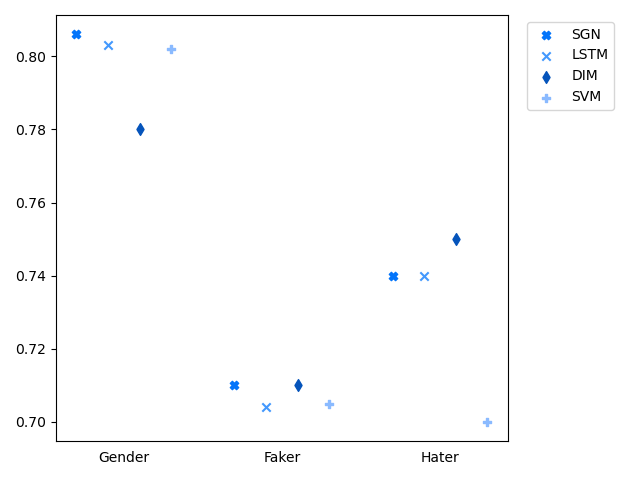
\includegraphics[width=0.45\textwidth]{images/compare_en.png}} \hspace{10mm}
		\subfigure[Idioma Español]{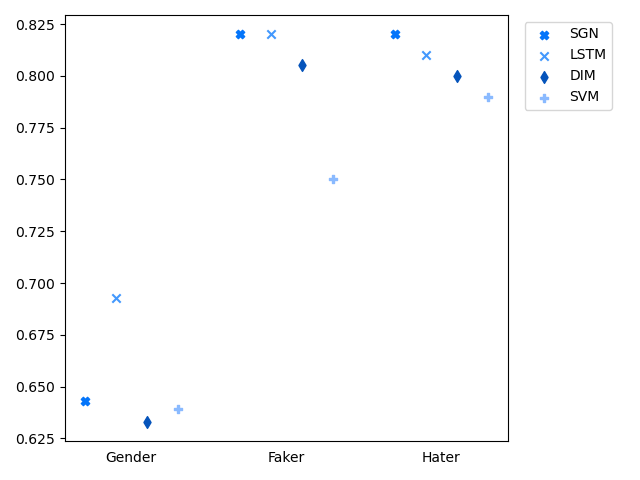
\includegraphics[width=0.45\textwidth]{images/compare_es.png}} 
		\caption[Resultados conjuntos de los modelos propuestos]{Resultados conjuntos de los modelos propuestos para el perfilado de autores en términos de \textit{accuracy}.}
		\label{compare}
	\end{figure}\\
	Con respecto a las ediciones de PAN 2020 y 2021, sobre la cual tenemos las colecciones completas y las tareas no fueron evaluadas de manera parcial, podemos decir que nuestros modelos alcanzan resultados competitivos y para el caso de PAN 2020, estos superan el desempeño medio del modelo mejor posicionado que empleó técnicas de Deep Learning \citep{giglou:2020} con un 74.5\% de \textit{accuracy} frente a 76.5\% alcanzado por el modelado del perfil basado en grafos propuesto en este trabajo bajo una arquitectura modular, además para el idioma español alcanzó el mejor \textit{accuracy} registrado en la competencia. 
		\begin{table}[thb!]
		\begin{center} 					 		
			\begin{tabular}{clccc} 
				\specialrule{.1em}{.05em}{.05em}
				Pos&Equipo&EN& ES&Avg.\\	
				\specialrule{.1em}{.05em}{.05em} 
				1&bolonyai20 \citep{buda:2020} & \textbf{0.7500}&0.8050&0.7775\\
				1&pizarro20 \citep{pizarro:2020}  &0.7350&\textbf{0.8200}&0.7775\\
				  &\textbf{SGN} & 0.7100 & \textbf{0.8200} & 0.7650\\
				  &\textbf{Att-LSTM} & 0.7040 & 0.8020&0.7620\\
				  &\textbf{DIM}& 0.7100 & 0.8050 &0.7575\\
				3&koloski20 \citep{koloski:2020a} &0.7150&0.7950&0.7550\\
				\multicolumn{5}{c}{...}\\
				8&babei20 \citep{giglou:2020} &0.7250&0.7650&0.7450\\
					\multicolumn{5}{c}{...}\\
				\specialrule{.1em}{.05em}{.05em} 
			\end{tabular}
			\caption[Resultados PAN 2020]{Resultados en \textit{accuracy} con respecto a los participantes oficiales (65) de la tarea ``Profiling Fake News Spreaders on Twitter''.}\label{pan20result}	
		\end{center}
	\end{table}		
	\\
	Para la tarea Profiling Hate Speech Spreaders on Twitter en PAN 2021, nuestra arquitectura SGN alcanzó un exactitud media de 78\% frente al 79\% alcanzado por el mejor modelo, sin embargo, cabe mencionar que nuestra modificación basada en el Método del los Impostores, alcanzó un desempeño superior para el idioma inglés con respecto a \citep{sinno:2021} (i.e.,73$+$1).
	\begin{table}[thb!]
		\begin{center} 					 		
			\begin{tabular}{clccc} 
				\specialrule{.1em}{.05em}{.05em}
				Pos&Equipo&EN& ES&Avg.\\	
				\specialrule{.1em}{.05em}{.05em} 
				1&SinnoDiNuovo \citep{sinno:2021} & 0.730&\textbf{0.850}&0.790\\
				2&MUCIC \citep{balouchzahi:2021}  &0.730&0.830&0.780\\
				2&UO-UPV \citep{tamayo:2021} &0.740&0.820&0.780\\
				&\textbf{SGN} & 0.740 & 0.820 & 0.780\\
				&\textbf{Att-LSTM} & 0.740 & 0.810&0.775\\
				&\textbf{DIM}& \textbf{0.750} & 0.800 &0.775\\
				4&andujar \citep{carracedo:2021}& 0.720 & 0.820 &0.770\\
				\multicolumn{5}{c}{...}\\
				\specialrule{.1em}{.05em}{.05em} 
			\end{tabular}
			\caption[Resultados PAN 2021]{Resultados en \textit{accuracy} con respecto a los participantes oficiales (67) de la tarea ``Profiling Hate Speech Spreaders on Twitter''.}\label{pan21result}	
		\end{center}
	\end{table}		
	\\
	Estos resultados, dan evidencia de la robustez de las arquitecturas modulares propuestas y en especial de la representación natural de los perfiles como datos no estructurados a través de los grafos.